\chapter{Introduction}
\label{chap:intro}

\section{Security Isolation for Applications}
\label{sec:intro:isolation}

In traditional operating systems, the security of an application is based on
trusting the whole system stack to always enforce the security policies.
The system stack needed to be trusted
--- counted as part of the {\em trusted computing base (TCB)}
--- includes the hardware (from CPUs to devices), operating systems, system libraries,
and even language runtimes that the application relies on.
If a vulnerability exists anywhere in the system stack,
attackers can exploit the vulnerability to bypass security mechanisms applied by the application,
compromising any security policies that application applies.

However, as the design of the hardware, operating systems, libraries and runtimes grows increasingly complex,
it becomes harder for system developers to eliminate the vulnerabilities
from the system stacks.
Theoretically, system developers can use debugging or formal verification
to assist or verify the elimination of vulnerabilities.
However, the formal technique cannot be proven perfect, and the latter requires tremendous effort to ensure its correctness
when the whole system stack is huge.

The existence of vulnerabilities in the trusted system stack especially affects applications that run in a multi-tenant environment, such as the {\em cloud}.
If there is only one tenant,
the application or user will always behaves benignly,
without actively attempting to discover or exploit any system vulnerabilities.
On the contrary, in a multi-tenant environment,
the application or user can share the same host with a malicious application or user,
who will act to compromise the system stack.
The problem can never be completely resolved by security checks,
because vulnerabilities can exist in the security logics,
and the attackers who succeed exploiting the vulnerabilities may bypass the checks.

To address the problem of system vulnerabilities, system researchers have engaged efforts in building more secure operating systems,
to isolate the consequence of compromised system stacks.
For instance,
micro-kernels, such as Exokernel or HiStar,
intend to reduce the TCB in the operating systems that are shared by applications.
The operating system components that are removed from the shared TCB are placed into a {\em library OS}, which operates in the userspace or even in the application processes.
If a malicious application attack its library OS,
the succeeded exploitation will only affect the very piece of library OS,
whereas other applications are isolated.
Because the complexity of the host kernel is significantly reduced,
it is easier to eliminate its vulnerabilities.

Another common approach of enforcing security isolation against malicious application to use virtualization.
With virtualization, the shared TCB among all the guests (or tenants)
are reduced to a minimal hypervisor,
and each guest will be running in an isolated virtual machine which loads a monolithic guest operating systems.
Similar as the applications isolated by library OSes, the exploitation that occurs in each guest OS will not affect other guests.

Either library OSes or virtual machines does not defend against two types of attacks.
The first type of attack is from the malicious host providers.
In cloud environment, the cloud providers are the third party that provides the host platforms for the users.
A malicious provider can load a modified kernels or hypervisors
into the hosts,
bypassing the security isolation enforced by library OSes or virtual machines.
Even without loading a malicious system stack,
the provider can still attack the hosts by physically launching attacks on the hardware, using techniques such as cold-boot attack~\citep{halderman09coldboot} or 
intrude the boot process using counterfeit peripheral devices.
Finally, system-level security isolation cannot defend against vulnerabilities
inside an application or a process
that can be exploited to attack the application itself.
To eliminate vulnerabilities in a complex modern applications is just as infeasible as eliminating vulnerabilties in the operating systems.



\section{Balancing Practicality and Security Isolation}
\label{sec:intro:practicality}


\section{Security Isolation for Native Linux Applications}
\label{sec:intro:graphene}

Existing library OSes provide single-process applications
with the qualitative benefits of virtualization
at a lower cost~\citep{porter11drawbridge,unikernels,baumann13bascule}.
These benefits include security isolation of mutually untrusting applications,
migration, and host platform compatibility.
%Library OSes move portions of
%OS kernel functionality into an application library.
In a library OS, the guest OS is essentially ``collapsed''
into an application library,
%% dp: too early for this nomenclature, I think
% \daniela{(a libraryOS instance)},
which implements the OS system calls and supporting data structures as library functions---mapping
high-level APIs onto
a few paravirtual interfaces to the host kernel.
Recent library OSes improve efficiency over full guest OSes by eliminating duplicated features
between the guest and host kernel,
such as the CPU scheduler, or
%eliminating guest-level multiplexing code, as the library OS supports only one application;
even compiling out unnecessary guest kernel APIs~\citep{unikernels}.
In total, this can reduce the memory requirements of running a single, isolated application
by orders of magnitude, and similarly
increase the number of applications which can run
on a single system~\citep{porter11drawbridge,unikernels}.
Library OSes ahve also proved
useful for porting legacy applications
onto new hardware platforms, such as Intel's SGX~\citep{baumann14haven}.
%% dp: This sentence seems a little premature
%In recent works, library OSes provide rich OS features for isolated contexts while the host OSes are untrusted

%% Library OSes reduce the memory requirements of running a self-contained,
%% isolated application process
%% %guest \daniela{I would replaced guest by "isolated process or group of processes (a libOS instance)''}
%% by orders of magnitude
%% In a cloud computing environment,
%% increasing the number of applications per server has enormous
%% economic benefits.
%% Even on a desktop or portable system, \libos{}es can reduce the overheads
%% of sandboxing untrusted code and running applications
%% designed for another OS.

%Because library OSes execute within a VM \daniela{this phrase does not read good to me because (i) it might imply the picoprocesses need hypervisor support, as misunderstood by reviewer 1 and (ii) you already emphasized the drawbacks of leveraging a VM} or lightweight process ({\em picoprocess}~\citep{xax}),
%library OSes execute with

%% dp: Daniela, great suggestion!  We need to make this situation seem more
%%     like the sky will fall without our help
A key drawback of recent library OSes, however,
is that they are limited to single-process applications.
Yet many applications, such as network servers and
shell scripts,
create multiple processes
for
performance scalability, fault isolation, and programmer convenience.
%These applications would benefit from the efficiency and security benefits
%of a library OS.
In order for the efficiency benefits of library OSes to be widely applicable,
especially for unmodified Unix applications,
%either applications must be rewritten to implement ad hoc coordination mechanisms, or
library OSes must  provide commonly-used multi-process abstractions,
such as fork,  signals, System V IPC, and exit notification.
To support multi-process abstractions, library OSes often have to rely on sharing OS states,
backed by the hosts' memory sharing features.
For example, Drawbridge~\citep{porter11drawbridge} cannot simulate process forking because copy-on-write memory sharing is not a platform-independent features.


%\begin{figure}[t!]
%\centering
%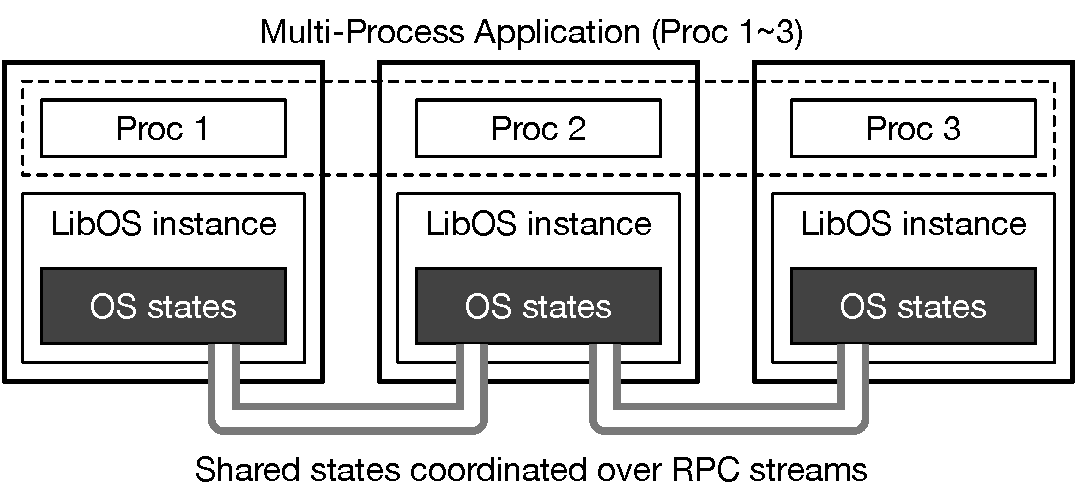
\includegraphics[width=0.75\linewidth]{graphene/figures/concept.pdf}
%\caption[Multi-process abstraction model of \sysname{} \libos{}]
%{Multi-process abstraction model of \sysname{} \libos{}. For each process of an application, a libOS instance will serve system calls and keep local OS states. States of multi-process abstractions are shared by coordinating over host-provided RPC streams, creating an illusion of running in single OS for the application.}
%%\vspace{-.1in}
%\label{fig:graphene:concept}
%\end{figure}

\begin{comment}
This paper describes {\bf \sysname{}},  a Linux-compatible library OS.
In \sysname{}, multiple libOS instances collaboratively implement
POSIX abstractions,
yet appear to the application
as a single, shared OS.
\sysname{} instances coordinate state using remote procedure calls (RPCs) over
host-provided byte streams (similar to pipes).
In a distributed POSIX implementation, placement of shared state and messaging complexity
are first-order performance concerns.
%We chose to shift implementation complexity into the library OS
%in order to uphold simple enforcement of security isolation in the host.
By coordinating shared states across libOS instances,
\sysname{} is able to create an illusion 
of running in a single OS
for multiple processes in an application (as figure~\ref{fig:concept}).

%Previous library OS designs ensured security isolation of independent applications,
%comparable to a VM, by keeping a relatively narrow host ABI.
%We selected the \sysname{}
%design because it strikes a unique balance between
%and robust, flexible security enforcement.

The \sysname{} design ensures security isolation of
mutually distrusting, multi-process
applications on the same host system.
Essential to this goal is
minimally expanding the host ABI to support multi-processing,
as well as leveraging RPCs as a natural point to mediate inter-libOS communication.
RPC coordination among \sysname{} instances can be dynamically disconnected, facilitating novel sandboxing
techniques.  For instance, we develop an Apache web server extension that, upon logging in a given user,
places the worker process's libOS in a sandbox with access to only that user's data.
We expect more nuanced degrees of trust are possible in future work.


The contributions of this paper are:
\begin{compactitem}
\item \sysname{}, a Linux library OS, which supports
  real-world, multi-process applications including a shell, web server,
  and compiler, which can be  efficiently checkpointed and migrated.
% \fixmetsai{We need to enable mulit-process checkpointing and migration}
% \daniela{the reviewers will be looking for that in the experiments section: "among hosts''}.
\item A framework for implementing multi-process APIs across cooperating library OS instances.
%\daniela{I would change to: "A thorough security analysis of \sysname{} isolation design'' You mention that you trust the reference momitor, so there is no security to
%be evaluated unless you guarantee the process is not vulnerable to exploits. We have not evaluated the security of the coordination design, only the isolation. To evaluate the security to the coordination design we have to look at possible race conditions and how they are dealt with.}
%\item Addressing additional challenges developing a robust Linux library OS, including copy-on-write fork.
\item A thorough evaluation of the overheads of \sysname{}.  Memory footprints are an order of magnitude
smaller than KVM, and several applications perform comparably to a Linux process.
\item A thorough analysis of \sysname{} security isolation.

%In the best case, the overhead of a large {\tt gcc} compilation on \sysname{} is only 3\%.

\end{compactitem}
\end{comment}

Graphene's design gives the user and system administrator a high degree of flexibility
in isolating arbitrary groups of unmodified application processes,
while upholding the efficiency and host compatibility benefits of recent library OSes.

%\fixmedp{After a complete draft is written, coalesce all goals and make sure they are addressed early on.  We are doing some scatter-shot motivation}

\section{Isolating Execution on Untrusted Hosts}
\label{sec:intro:graphene-sgx}



\section{Combining Isolated Execution with Language-based Protection}
\label{sec:intro:graphene}


\section{Extended Topics}

\subsection{Decoupling Performance and Compatibility Requirement}

\subsection{Revisiting Compatibility Requirement}

\section{Future Works}